\documentclass[11pt,a4paper,notitlepage,onecolumn]{article}
\usepackage[german]{babel}
\usepackage[utf8]{inputenc}
\usepackage{graphicx}
\title{Aufgabe5\_3}
\author{Robin Nehls, Yves Müller\\
  Freie Universit\"at Berlin\\
  nehls@spline.de uves@spline.de }
\date{}
\begin{document}

\maketitle

\paragraph{}

\begin{figure}
\centering
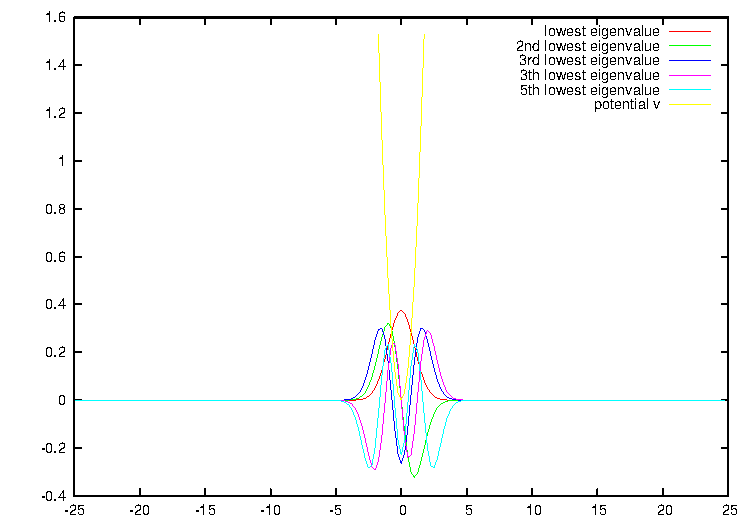
\includegraphics[width=\textwidth]{aufgabe3-normal.pdf}
\caption{\em \small plott of the lowest 5 eigenvalues}
\end{figure}

\paragraph{Choosing smaller harmonic potentials}
When computing the hamiltonien with smaller potentials, we meet several new 
problems. First of all our solutions have much smaller absolute values, but
our machine accuraccy keeps still the same, wich leavs might lead to bigger
relative Error. On the other hand we have to increase the our N or increase 
our \delta x, in order to be able to plot all eigenfunctions completle,
wich results in more operations (where $O(n)=n^3$), or lesser accuracy.


\begin{figure}
\centering
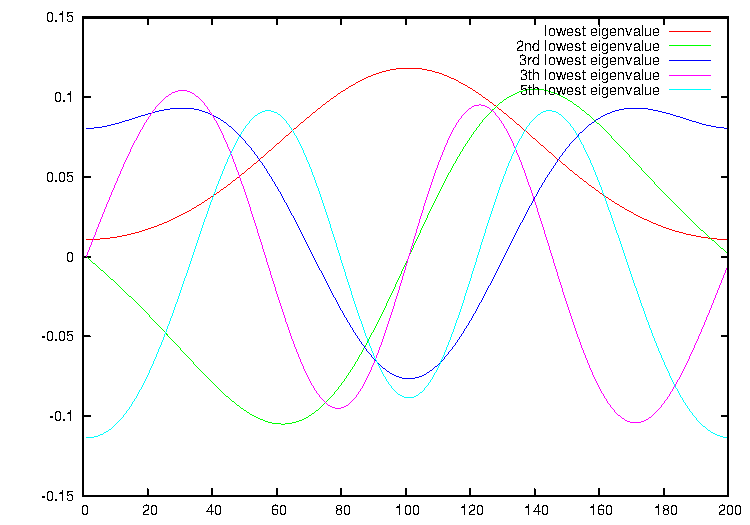
\includegraphics[width=\textwidth]{aufgabe3-lowpot.pdf}
\caption{\em \small plot with lower harmonic potential}
\end{figure}

\end{document}
